\documentclass{article}
\usepackage[T2A]{fontenc}
\usepackage[utf8]{inputenc}
\usepackage[english, russian]{babel}

\usepackage{geometry}
\geometry{a4paper, top=1cm, bottom=2cm, left=1.5cm, right=1.5cm}

\usepackage{indentfirst}
\usepackage{amssymb,amsfonts,amsmath}
\usepackage{cite,enumerate}
\usepackage[pdftex,colorlinks,unicode,bookmarks]{hyperref}

\usepackage{floatrow}
\usepackage{caption}
\usepackage{subcaption}
\usepackage{multirow}
\usepackage[table]{xcolor}
\usepackage{graphicx}

\title{
        Воспроизведение результатов известных статей в \href{https://github.com/illusionww/py_graphs}{py\_graphs} и анализ сравнения.
}
\author{Владимир Ивашкин}

\begin{document}

\maketitle


\section*{Введение}
Для того, чтобы проводить эксперименты с метриками, нам нужно быть уверенными, что метрики не содержат ошибок. В прошлом мы убеждались, что ошибки имеют место быть.
Я воспроизвел результаты четырех статей и оформил это в виде тестов к моему коду. Теперь после любых значимых изменений я буду запускать эти тесты и расследовать возникающие расхождения. Так победим.

Этот текст нужен в том числе и мне, чтобы не забыть, что именно я делал и чем руководствовался.

\tableofcontents

\section{Pavel Chebotarev:\\
         Studying new classes of graph metrics}
Ссылка: \url{https://arxiv.org/abs/1305.7514}

\subsection{Figure 1}
В Fig. 1 на графе ``цепочка'' показаны расстояния между вершинами в зависимости от метрики. Расстояния здесь нормированы на $D_{12} + D_{23} + D_{34} = 3$.
Достаточно будет сравнивать расстояния $D_{12}, D_{23}, D_{13}, D_{14}$.

Вначале результаты не сходились, но потом выяснилось следующее:
\begin{itemize}
  \item В моем коде из всех ядер, перед тем, как превращать их в расстояния, брался корень. Мы обсуждали, что это нужно для Communicability, но в итоге это было включено везде. В этом причина, почему раньше результаты не совпадали с этой работой;
  \item Для Communicability взятие корня все-таки нужно, в этом случае результаты совпадают по всем метрикам.
\end{itemize}

\begin{table}[H]
\centering
\caption{Comparison with ``Studying new classes of graph metrics'', Figure 1}
\label{}
\begin{tabular}{rr|cccc}
             &      & $D_{12}$ & $D_{23}$ & $D_{13}$ & $D_{14}$ \\
             \hline
SP           & true & 1.000 & 1.000 & 2.000 & 3.000 \\
             & test & 1.000 & 1.000 & 2.000 & 3.000 \\
             \hline
R            & true & 1.000 & 1.000 & 2.000 & 3.000 \\
             & test & 1.000 & 1.000 & 2.000 & 3.000 \\
             \hline
Walk         & true & 1.025 & 0.950 & 1.975 & 3.000 \\
             & test & 1.025 & 0.950 & 1.975 & 3.000 \\
             \hline
logFor       & true & 0.959 & 1.081 & 2.040 & 3.000 \\
             & test & 0.959 & 1.081 & 2.041 & 3.000 \\
             \hline
For          & true & 1.026 & 0.947 & 1.500 & 1.895 \\
             & test & 1.026 & 0.947 & 1.500 & 1.895 \\
             \hline
SqResistance & true & 1.000 & 1.000 & 1.414 & 1.732 \\
             & test & 1.000 & 1.000 & 1.414 & 1.732 \\
             \hline
Comm         & true & 0.964 & 1.072 & 1.492 & 1.564 \\
             & test & 0.964 & 1.072 & 1.492 & 1.564 \\
             \hline
pWalk 4.5    & true & 1.025 & 0.950 & 1.541 & 1.466 \\
             & test & 1.025 & 0.950 & 1.541 & 1.466 \\
             \hline
pWalk 1.0    & true & 0.988 & 1.025 & 1.379 & 1.416 \\
             & test & 0.988 & 1.025 & 1.379 & 1.416
\end{tabular}
\end{table}

\subsection{Pavel Chebotarev: The Walk Distances in Graphs, Table 1}
Также я воспроизвел результаты из Table 1 в Pavel Chebotarev: The Walk Distances in Graphs (ссылка: \url{https://arxiv.org/abs/1103.2059}). Скорее всего, они основаны на тех же результатах, что уже были в таблице выше, но дополнительные проверки не помешают.

\begin{table}[H]
\centering
\caption{Comparison with ``The Walk Distances in Graphs'', Table 1}
\label{my-label}
\begin{tabular}{rr|ccc}
          &      & $D_{12} / D_{23}$ & $(D_{12}+D_{23}) / D_{13}$ & $D_{14} / D_{12}$ \\
          \hline
SP        & true & 1.000 & 1.000 & 1.500 \\
          & test & 1.000 & 1.000 & 1.500 \\
          \hline
R         & true & 1.000 & 1.000 & 1.500 \\
          & test & 1.000 & 1.000 & 1.500 \\
          \hline
Walk      & true & 1.080 & 1.000 & 1.520 \\
          & test & 1.080 & 1.000 & 1.519 \\
          \hline
logFor    & true & 0.890 & 1.000 & 1.470 \\
          & test & 0.887 & 1.000 & 1.470 \\
          \hline
For       & true & 1.080 & 1.320 & 1.260 \\
          & test & 1.083 & 1.316 & 1.263 \\
          \hline
pWalk 4.5 & true & 1.080 & 1.280 & 0.950 \\
          & test & 1.079 & 1.281 & 0.951 \\
          \hline
pWalk 1.0 & true & 0.960 & 1.460 & 1.030 \\
          & test & 0.964 & 1.459 & 1.027 
\end{tabular}
\end{table}

Видим, что с этими тестами тоже все ок. В последнем разделе я привожу сводную таблицу, где показываю, что именно было покрыто воспроизведением результатов каждой статьи.


\section{Ilkka Kivim{\"a}ki, Masashi Shimbo, Marco Saerens:\\
         Developments in the theory of randomized shortest paths with a article comparison of graph node distances}
Ссылка: \url{https://arxiv.org/abs/1212.1666}

\subsection{Figure 2}
Здесь исследуется поведение метрик RSP, FE, pRes, logFor, SP-CT при изменении их параметров в заданном интервале для графа ``треугольник с хвостом''. Можно исследовать всю кривую, для простоты возьмем только крайние точки: слева отношение $\Delta_{12}/\Delta_{23}$ равно 1.5, справа --- 1.0.

Раньше здесь были проблемы у logFor но после того, как я перестал брать корень из матрицы расстояний, все результаты сошлись:

\begin{table}[H]
\centering
\caption{Comparison with ``Developments ...'', Figure 2}
\label{my-label}
\begin{tabular}{rll|cc|c}
       &         &        & \multicolumn{3}{c}{$D_{12} / D_{23}$} \\
border & measure & param  & test   & true & diff   \\
       \hline
left   & CT      & --     & 1.5    & 1.5  & 0      \\
       & logFor  & 500.0  & 1.4975 & 1.5  & 0.0025 \\
       & RSP     & 0.0001 & 1.4992 & 1.5  & 0.0008 \\
       & FE      & 0.0001 & 1.4996 & 1.5  & 0.0004 \\
       \hline
right  & SP      & --     & 1      & 1    & 0      \\
       & logFor  & 0.01   & 1.0011 & 1    & 0.0011 \\
       & RSP     & 20.0   & 1      & 1    & 0      \\
       & FE      & 20.0   & 0.9834 & 1    & 0.0166
\end{tabular}
\end{table}

\subsection{Table 2 с оптимальными значениями из Table 1}
Здесь проверяется качество (по NMI*100) кластеризации методом kMeans графов из датасета Newsgroups. Кернелы: RSP, FE, logFor, SP-CT, SCT. Результаты совпадают со статьей для всех метрик, кроме SP-CT. Для последней результат очень плох: в статье ожидается качество порядка 70-80 NMI*100, по факту что SP, что CT дают 0.2-3 NMI*100. SP-CT применяется с параметром 1, то есть чистый SP.

\begin{table}[H]
\centering
\caption{Comparison with ``Developments ...'', Table 2}
\label{my-label}
\begin{tabular}{rr|rrrrrr}
         &      & n2cl1  & n2cl2  & n2cl3  & n3cl1  & n3cl2  & n3cl3 \\
         \hline
         & test & 79.443 & 57.914 & 81.070 & 77.092 & 76.797 & 75.520 \\
RSP      & true & 84.500 & 58.700 & 81.000 & 76.600 & 77.000 & 76.500 \\
         & diff & 5.057  & 0.786  & 0.070  & 0.492  & 0.203  & 0.980  \\
         \hline
         & test & 79.443 & 57.917 & 81.070 & 76.619 & 77.980 & 75.131 \\
FE       & true & 80.700 & 58.700 & 81.100 & 76.200 & 78.300 & 77.000 \\
         & diff & 1.257  & 0.783  & 0.030  & 0.419  & 0.320  & 1.869  \\
         \hline
         & test & 81.846 & 60.952 & 76.988 & 78.376 & 75.010 & 75.121 \\
logFor H & true & 83.100 & 58.800 & 75.000 & 75.400 & 75.500 & 74.400 \\
         & diff & 1.254  & 2.152  & 1.988  & 2.976  & 0.490  & 0.721  \\
         \hline
         & test & 0.219  & 0.147  & 0.201  & 0.315  & 0.334  & 0.295  \\
SP-CT K  & true & 65.200 & 51.200 & 85.900 & 74.200 & 62.600 & 71.500 \\
         & diff & \cellcolor{red!25} 64.981 & \cellcolor{red!25} 51.053 & \cellcolor{red!25} 85.699 &
                  \cellcolor{red!25} 73.885 & \cellcolor{red!25} 62.266 & \cellcolor{red!25} 71.205 \\
         \hline
         & test & 81.105 & 54.616 & 78.440 & 77.922 & 72.276 & 75.409 \\
SCT H    & true & 81.600 & 56.800 & 79.600 & 77.300 & 73.000 & 75.900 \\
         & diff & 0.495  & 2.184  & 1.160  & 0.622  & 0.724  & 0.491  
\end{tabular}
\end{table}


\section{Felix Sommer, Fran{\c c}ois Fouss, Marco Saerens:\\
         Comparison of Graph Node Distances on Clustering Tasks}
Ссылка: (не находил в открытых источниках)

Здесь нас интересует Table 3 с оптимальными значениями из Table 2.
Метрики: CCT, FE, logFor, RSP, SCT, SP.
Датасеты: football, newsgroups, polblogs, zachary.
Проблемы: CCT не работает для football, на polblogs не работает ничего, видимо из-за большого размера. Для SP не проходят почти все тесты.

\begin{table}[H]
\centering
\caption{Comparison with ``Comparison of Graph Node Distances on Clustering Tasks'', Table 3}
\label{my-label}
\begin{tabular}{rr|rrrrrrrr}
       &      & n2cl1 & n2cl2 & n2cl3 & n3cl1 & n3cl2 & n3cl3 & zachary & football \\
       \hline
       & test & 0.794 & 0.598 & 0.758 & 0.784 & 0.758 & 0.746 & 1.000   & \cellcolor{red!25} error    \\
SCCT   & true & 0.794 & 0.582 & 0.758 & 0.778 & 0.762 & 0.746 & 1.000   &          \\
       & diff & 0.000 & 0.016 & 0.000 & 0.006 & 0.004 & 0.000 & 0.000   &          \\
       \hline
       & test & 0.797 & 0.645 & 0.811 & 0.781 & 0.763 & 0.764 & 1.000   & 0.862    \\
FE     & true & 0.805 & 0.591 & 0.811 & 0.781 & 0.797 & 0.771 & 1.000   & 0.906    \\
       & diff & 0.008 & 0.054 & 0.000 & 0.000 & 0.034 & 0.006 & 0.000   & 0.045    \\
       \hline
       & test & 0.831 & 0.622 & 0.769 & 0.746 & 0.745 & 0.752 & 1.000   & 0.895    \\
logFor & true & 0.838 & 0.584 & 0.748 & 0.753 & 0.758 & 0.749 & 1.000   & 0.903    \\
       & diff & 0.007 & 0.038 & 0.021 & 0.007 & 0.014 & 0.003 & 0.000   & 0.008    \\
       \hline
       & test & 0.797 & 0.635 & 0.785 & 0.781 & 0.786 & 0.725 & 1.000   & 0.895    \\
RSP    & true & 0.797 & 0.580 & 0.796 & 0.781 & 0.776 & 0.730 & 1.000   & 0.909    \\
       & diff & 0.000 & 0.055 & 0.011 & 0.000 & 0.010 & 0.005 & 0.000   & 0.014    \\
       \hline
       & test & 0.820 & 0.625 & 0.824 & 0.753 & 0.723 & 0.765 & 1.000   & 0.845    \\
SCT    & true & 0.817 & 0.552 & 0.786 & 0.773 & 0.728 & 0.763 & 1.000   & 0.811    \\
       & diff & 0.002 & 0.073 & 0.039 & 0.020 & 0.005 & 0.002 & 0.000   & 0.033    \\
       \hline
       & test & 0.003 & 0.003 & 0.009 & 0.003 & 0.021 & 0.006 & 0.677   & 0.861    \\
SP     & true & 0.654 & 0.516 & 0.859 & 0.743 & 0.625 & 0.720 & 1.000   & 0.858    \\
       & diff & \cellcolor{red!25} 0.651 & \cellcolor{red!25} 0.513 & \cellcolor{red!25} 0.850 &
                \cellcolor{red!25} 0.740 & \cellcolor{red!25} 0.603 & \cellcolor{red!25} 0.714 & \cellcolor{yellow!25} 0.323   & 0.004   
\end{tabular}
\end{table}

Все проблемы минорные, кроме SP. SP выдает плохое качество в обоих статьях.
Как работает SP:
\begin{itemize}
  \item Вызывается функция shortest\_path() из scipy (проверял на маленьких графах, выдает правильные результаты. Также были тесты по статье ``Studying new classes of graph metrics'', там тоже результаты верные)
  \item (опционально) Применяется нормализация, чтобы параметр адекватно смешивал SP и CT
  \item Применяется $D \rightarrow K$ преобразование
\end{itemize}

Больше ничего тут нет. Проблемы с $D \rightarrow K$ тоже быть не может, ведь RSP и FE преобразуются этой же формулой. Без нормализации наблюдаем ту же проблему. Если заменить kMeans на Ward, то качество тоже не растет --- значит проблема не специфична для кластеризатора.

Что еще интересно, с уменьшением размеров графа качество кластеризации растет (видим, что на football получилось приличное качество). Похоже на проблему у CT, описанную в Getting lost in space. Очень странно, тем более странно, что проблема коснулась только SP. По CT нет результатов для больших графов, может у CT тоже есть такая проблема?


\section{Konstantin Avrachenkov, Pavel Chebotarev, Dmytro Rubanov:\\
         Kernels on Graphs as Proximity Measures}
Ссылка: \url{https://hal.inria.fr/hal-01647915/document}

Помимо статьи, здесь у наc был доступен код. Я добавил все метрики из этого кода к себе в репозиторий. Часть метрик у нас уже была реализована, часть --- нет.
Исследование можно разделить на две части: сравнение реализаций Рубанова и моих для совпадающих мер, и воспроизведение результатов кластеризации из статьи.

\subsection{Сравнение реализаций на всем пространстве параметров}
Сравнивались результаты для одного простого графа на всем пространстве параметров. Метрики: Walk, logComm, logHeat, Forest. Метрики совпали с точностью  $0.0001$.

Кажется, тут есть некоторые проблемы с наименованиями: в статье метрики выглядят как plain и только в коде понятно, что метрики логарифмируются. Но так как у нас код был, проблем не возникло.

\subsection{Balanced Model}
Сравнивались результаты из секции ``Balanced Model'' для метрик Walk, logComm, logHeat, Forest (мои реализации), а также Normalized Heat, Personalized PageRank, Modified Personalized PageRank, Heat Personalized PageRank (реализации Рубанова). Сравнение сделано для сгенерированных графов.

Вначале у результатов были расхождения: одни и те же реализации давали качество в среднем на 0.004 хуже, чем в статье.

Сначала я заподозрил генератор графов: несмотря на то, что в основе лежит одна и та же идея, реализации дают разные результаты. Насколько я понял, самое важное отличие --- они проверяют связность графа и подбирают только связные. Использование генератора немного подняло результаты, но не настолько, чтобы считать тесты пройденными.

После этого я решил использовать для теста именно те графы, на которых считал Рубанов: он зафиксировал, на каких именно графах он получил результаты. И ничего не совпало.

Внимательнее посмотрев код, я нашел важное отличие от нашего эксперимента: мы стараемся найти наилучший параметр, который подходил бы всем графам, и смотрим на качество при этом параметре. В коде Рубанова же наилучший параметр находится отдельно для каждого графа и по лучшему качеству для каждого графа проводится усреднение. Переписав метод оценки параметра, мне удалось получить такие же результаты. Некоторые расхождения все же есть, можно списать их на недетерминированную работу спектральной кластеризации.

\begin{table}[H]
\centering
\caption{Comparison with ``Kernels on Graphs as Proximity Measures'', Balanced Model}
\label{my-label}
\begin{tabular}{r|rrr}
                               & test   & true   & diff   \\
                               \hline
Katz                           & 0.0071 & 0.0072 & 0.0001 \\
Estrada                        & 0.0086 & 0.0084 & 0.0002 \\
Heat                           & 0.0068 & 0.0064 & 0.0004 \\
Normalized Heat                & 0.0067 & 0.0066 & 0.0001 \\
Regularized Laplacian          & 0.0071 & 0.0072 & 0.0001 \\
Personalized PageRank          & 0.0071 & 0.0073 & 0.0002 \\
Modified Personalized PageRank & 0.0072 & 0.0072 & 0.0000 \\
Heat Personalized PageRank     & 0.0082 & 0.0074 & 0.0008
\end{tabular}
\end{table}

\section{Тесты по другим источникам}

\subsection{Репозитории GitHub}
Я попробовал найти другие реализации shortest path --- не помогло. Попробовал найти сразу shortest path kernel и нашел здесь: \url{https://github.com/gmum/pykernels}, но результат все такой же плохой.

Также искал другие реализации мер для того, чтобы расширить количество тестов. Наткнулся на вот этот репозиторий: \url{https://github.com/jmmcd/GPDistance}. Здесь есть более сложные реализации RSP и FE. Насколько я понял, они защищены от случаев вроде тех, когда граф не связный (защищены от деления на 0 при вычислении Pref). Я реализовал тесты из этого репозитория и увидел, что RSP и FE из этого репозитория выдают значения на более широком диапазоне параметров, чем мои варианты, сделанные строго по формулам из статей. Я заменил свои версии версиями из репозитория и они проходят все наши тесты. В частности, таблицы выше содержит результаты с обновленными мерами.

\subsection{Luh Yen, Francois Fouss, Christine Decaestecker, Pascal Francq, Marco Saerens: \\
            Graph Nodes Clustering based on the Commute-Time Kernel}
Итак, мне нужно больше статей про SP и CT, в которых были бы результаты, с которыми я мог бы сравниваться. В этой статье нас интересует Table 1, колонки $K_{CT}$ k-means. Здесь используется известный нам датасет Newsgroups и известные нам метрики RI (в таблице ``class. rate'' соответствует 100*RI) и ARI.

Получаем качество, близкое к 0 по ARI, то есть случайное гадание. Это совсем не похоже на результаты, описанные в статье, значит у нас неправильно реализованы и SP, и CT.
Проверяю эксперимент, заменяя кернел на logFor при параметре 0.95 -- оптимальный параметр для Newsgroup и получаю качество, почти достигающее заявленных значений.

У меня есть непонимание насчет того, что значит $L+$. По идее $+$ это взятие псевдообратной матрицы методом Мура-Пенроуза, в python есть такая функция. Но в Forest, который по идее должен быть обобщением CT, $(I + tL)^{-1}$, то есть добавляется I. Поэлементно логарифмированная $(I + L)^{-1}$ дает хорошее качество (это logFor при параметре 1), при убирании $log$ качество падает до нуля по ARI.

Взятие корня из CT тоже поправляет метрики. Это воспроизводится и на kMeans (который был проверен выше), и на Ward.


\section{Сравнение генератора графов с версией Рубанова}

Генератор из кода Рубанова делит список вершин на отрезки, соответствующие классам, без перемешивания. Потом из каждого класса последовательно берутся элементы, для каждого из них бросается монетка насчет связи с элементами из этого же класса вперед (вперед по списку вершин, чтобы избежать повторений) и для всех элементов следующих классов.

\begin{figure}[H] %tb
	\begin{minipage}{.5\textwidth}
		\centerline{
			\includegraphics[width=.9\linewidth]{pictures/pg-vs-rubanov/pgward_pout01_averaging200.png}
		}
	\end{minipage}%
	\begin{minipage}{.5\textwidth}
		\centerline{
			\includegraphics[width=.9\linewidth]{pictures/pg-vs-rubanov/pgward_pout01_averaging200_2.png}
		}
	\end{minipage}%
\caption{\label{f_Rcur}Ours vs Rubanov, ours Ward, $p_{out}=0.1$ averaging 200 (two runs)}
\end{figure}

Кажется, это должно работать так же, как и моя схема. Раз его решение и мое прошлое решение дают результаты ниже, чем мой текущий генератор, значит мой текущий генератор работает неправильно.

А что если перепроверить вероятности, возвращаемые генераторами, напрямую? Выйдет неплохой тест.
Но нет, все в порядке, у обоих генераторов хорошее распределение. Провел тест для $p_{in} = 0.3, p_{out} = 0.1$ при усреднении в 1000 графов.

Моя модель: $p_{in} = 0.2996, p_{out} = 0.1007$, модель Рубанова $p_{in} = 0.3003, p_{out} = 0.1002$.

Окей, я написал еще один генератор, проще чем оба предыдущие. Новый генератор практически сошелся с генератором Рубанова. Ниже график с усреднением по 20 графам.

\begin{figure}[H]
	\includegraphics[width=.75\linewidth]{pictures/pg-vs-rubanov/three-gen.png}
	\caption{\label{f_vs2} Сравнение трех генераторов}
\end{figure}

Здесь получается однозначный вывод: мой старый генератор показывает завышенные результаты по отношению к более простому (без возможности проставлять размеры классов и матрицу вероятностей) и генератору Рубанова. Это связано либо с генерацией случайных значений матрицами вместо поэлементных, либо с ошибкой, которую я не могу найти. Хорошие новости: этого бага не было на момент публикации. Буду использовать один из двух генераторов.


\section{Сравнение кластеризаторов Ward и KMeans с реализациями из Sklearn}
Здесь я построил графики ARI от параметра метрики для основного набора метрик для двух разных реализаций Ward и KMeans: самодельные, которые мы использовали до сих пор, и реализации, предложенные Николаем Козырским.

\begin{figure}[H]
	\includegraphics[width=.75\linewidth]{pictures/pg-vs-sklearn/pout01_averaging200.png}
	\caption{\label{f_vs2} Ours vs Sklearn $p_{out}=0.1$ averaging 200}
\end{figure}

\begin{figure}[H]
	\includegraphics[width=.75\linewidth]{pictures/pg-vs-sklearn/pout01_averaging500.png}
	\caption{\label{f_vs2} Ours vs Sklearn $p_{out}=0.1$ averaging 500}
\end{figure}

Видим, что все графики не совпадают. Версия kMeans, которую мы использовали раньше, мне не нравилась, и здесь она показала себя значительно хуже всех. Хорошо, будем использовать версию из sklearn. Расстраивает, что версии Ward тоже различаются. Я могу ручаться за текущую реализацию Ward, писал ее по статье и она дает хорошие результаты. Но, почему-то, при других параметрах. 

Еще странно, что kMeans и Ward из sklearn показывают наилучшее качество на одних и тех же параметрах. Хотя, может быть, это как раз логично? Мол, оптимальный параметр для метрики объективен и не нужно подбирать его для каждого метода кластеризации?

У меня есть некоторое недоверие к методам из sklearn, в документации не написано, что они используются именно для кернелов. Вдруг они оптимизируются при других параметрах, потому что при них кернел больше похож на матрицу расстояний? Решил провести такой эксперимент: взять самый простой граф и посмотреть качество на нем.

\begin{figure}[H]
	\includegraphics[width=.3\linewidth]{pictures/pg-vs-sklearn/examplegraph.png}
	\caption{\label{f_vs2} Матрица смежности для простого графа}
\end{figure}

\begin{figure}[H]
	\includegraphics[width=.75\linewidth]{pictures/pg-vs-sklearn/singlegraph-averaging1.png}
	\caption{\label{f_vs2} Зависимость качества от параметра метрики для простого графа}
\end{figure}

\begin{figure}[H]
	\includegraphics[width=.75\linewidth]{pictures/pg-vs-sklearn/singlegraph-averaging100.png}
	\caption{\label{f_vs2} Зависимость качества от параметра метрики, усредненная на ста запусках для одного и того же простого графа}
\end{figure}

Видим здесь, что kMeans, который мы использовали раньше, нестабильно работает, и дает качество близкое к нулю в при случайных значениях параметра метрики. Усреднение показывает случайный характер этого. Остальные методы кластризации справились с задачей. Значит ли это, что они все работают для кернелов?

Еще одна идея: может быть, эти функции принимают строчки ядра как вектора признаков? Возможно ли, что в такие кластеризаторы тоже дают хорошее качество, но на других значениях параметров?

Графики выше строились по графам, сгенерированным моей моделью, но в предыдущей секции мы увидели, что это плохая модель и мы ее использовать не будем. Вот график для $p_{in} = 0.3, p_{out} = 0.15$ на графах модели Рубанова:


\begin{figure}[H]
	\includegraphics[width=.75\linewidth]{pictures/pg-vs-sklearn/rubanovs-generator.png}
	\caption{\label{f_vs2}}
\end{figure}

Эта картинка гораздо приятнее выглядит. Здесь почти везде видна корреляция трех графиков. Можно предположить, что моя реализация Ward правильная, но наивная, поэтому она проигрывает.


\section{Вопросы по reject curves}

\subsection{}
\textit{Привлекает внимание Heat (p.4). Частично мы это уже обсуждали. Самое невероятное - что при $p_{out} = 0.1$ для абсолютного большинства графов Heat разделяет классы лучше, чем при $p_{out} = 0.05$. Т.е. при $0.05$ просто нет графов, кот. разделяются так же хорошо, как большинство при $0.1$. Как это возможно? Или лучшие графы при $0.05$ дают переполнение и отбрасываются?}
	
\textit{При $p_{out} = 0.1$ есть буквально 5 патологических графов. Что с ними происходит, почему Heat не справляется? Можно было бы предположить, что это графы, где плотность межклассовых связей существенно отклоняется вверх от $0.1$.}
	
\textit{При $p_{out} = 0.15$ - единственное широкое равномерное разнообразие - от хорошего до плохого разделения классов. Т.е. Heat необычайно чувствителен к каким-то колебаниям в графе. Некоторые другие меры, например, Walk дают больший разброс при низком $p_{out}$. Совершенно удивительно, что в среднем при этом Heat справляется примерно так же, как при $p_{out} = 0.05$.}

Похоже, у меня есть ответ на этот вопрос. 

Во-первых, был нестабильный генератор. Пересчитанные reject curves для нового генератора:

\begin{figure}[H]
	\includegraphics[width=.37\linewidth]{pictures/questions/1/rq_all.png}
	\caption{\label{f_vs2}}
\end{figure}


\begin{figure}[H] %tb
	\begin{minipage}{.5\textwidth}
		\centerline{
			\includegraphics[width=.9\linewidth]{pictures/questions/1/rq_avg_all.png}
		}
	\end{minipage}%
	\begin{minipage}{.5\textwidth}
		\centerline{
			\includegraphics[width=.9\linewidth]{pictures/questions/1/rq_avg_4.png}
		}
	\end{minipage}%
\caption{\label{f_Rcur} Усреднение}
\end{figure}

Во-вторых, построение тут ведется в два этапа: сначала мы для сотни сгенерированных графов определяем оптимальные параметры (используя Ward, потому что определить качество без использования кластеризатора нельзя), потом генерируем новые графы и строим графики для определенных ранее параметров. Так как параметр не зафиксирован, при плохом усреднении мы можем получить плохие параметры мер. Вот пример зависимости качества от параметра:

\begin{figure}[H]
	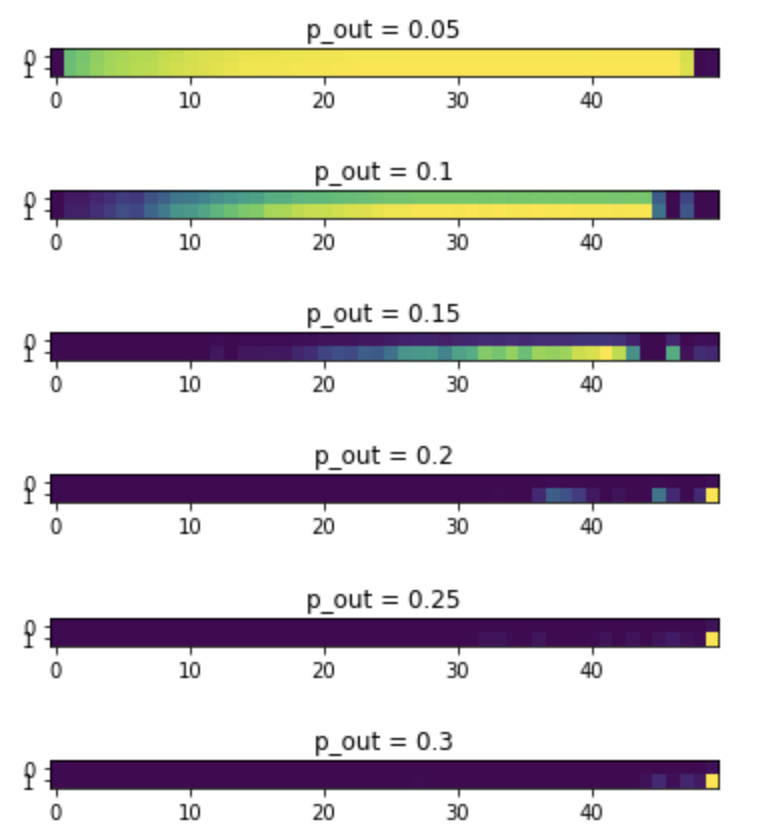
\includegraphics[width=.5\linewidth]{pictures/questions/1/quality.jpeg}
	\caption{\label{f_vs2} Heat}
\end{figure}

Здесь по оси x -- параметр от 0 до 1 (считал с шагом 0.02, поэтому шкала от 0 до 50), яркость обозначает качество (желтый -– 1 по ARI, синий -- 0), первая строчка -- абсолютный результат, вторая – относительный, деленный на максимум в этой строке. 

Здесь видно, например, что оптимальный параметр для Heat для всех параметров $p_{out} = 0.8$, в последних трех строчках видно, что при любом параметре качество близкое к нулю, но максимумом будет параметр близкий к единице, там где Heat вообще, скорее всего, не существует.

Итак, если для всех параметров генерации графов выбрать параметр Heat 0.8, то будут вот такие графы и вот такое усреднение:

\begin{figure}[H]
	\includegraphics[width=\linewidth]{pictures/questions/1/08_all.png}
	\caption{\label{f_vs2} Графы}
\end{figure}

\begin{figure}[H]
	\includegraphics[width=.5\linewidth]{pictures/questions/1/08_avg.png}
	\caption{\label{f_vs2} Усреднение}
\end{figure}  

\subsection{}
\textit{Интересно, что $Comm$ при $p_{out} = 0.05$ обгоняет $logComm$. Еще лучше $SCCT$ -- практически абсолютный результат.}

Теперь не обгоняет =)


\subsection{}
\textit{Интересен вертикальный участок справа у SP. Если это строится так, как я представляю, значит, при любом $p_{out}$ ровно $0.25$ пар "одноклассников" имеют максимальное расстояние, недостижимое для разноклассников. Чему оно равно? 3?}

Да, 3. Вот распределение для одного из графов, сгенерированных для $p_{out} = 0.05$
\begin{figure}[H]
	\includegraphics[width=.75\linewidth]{pictures/questions/3/download.png}
	\caption{\label{f_vs2} Распределения значений матрицы расстояний SP для одного графа}
\end{figure}
Кстати, получается что здесь reject curve строится несколько произвольно: точки резких перегибов на своих местах, а вот кривая между ними зависит от порядка вершин в матрице смежности. Это может касаться и других мер: если мы не перемешиваем вершины в матрице смежности, то мы склонны всегда занижать или завышать качество, определенное через reject curve. Сейчас именно такой вариант: оба генератора, прошедшие проверку, не перемешивают вершины.
Тут есть и еще один вопрос: если значения у SP всего три, то откуда вмозможны три излома? Может быть, я докидываю диагональные элементы, у которых SP=0?


\subsection{}
\textit{Еще было бы интересно построить матрицу ранговых корреляций мер по множеству случайных графов.
Тогда будет ясно, какие меры наиболее близки, какие далеки в смысле порядка.}
К сожалению, я не знаю, как это правильно нужно делать, нашел примеры здесь: \url{http://cito-web.yspu.org/link1/metod/theory/node42.html}. Понял это так:
\begin{enumerate}
\item У нас есть $n$ измерений, для каждого измерения мы ранжируем меры по результатам
\item Для каждой пары мер считаем сумму квадратов разностей $\sum_{M_1M_2} d_i^2$
\item По формуле $r_{M_1M_2} = 1 - \frac{6 * \sum_{M_1M_2} d_i^2}{(n-1)n(n+1}$ (корреляция Спирмена) считаем элементы матрицы корреляций
\end{enumerate}

Очень просто посчитать такое для нашей таблицы рангов 


\subsection{}
\textit{Берем функцию распределения (кумулятивную, S-образная кривая) ненулевых внутриклассовых расстояний и вычитаем из нее функцию распределения межклассовых расстояний. Должна получиться n-образная кривая. Преимущество ее, например, в том, что она показывает интервал, на котором распределено расстояние.}

\textit{Для эффектности ее можно продифференцировать - тогда экстремумы покажут точки сосредоточения тех и других расстояний. Аналогично можно делать для kernels - будет видно, на distances основной эффект оказывают диагональные или недиагональные эл-ты kernels. (Кстати, недостаток commute time, возможно, - в доминировании эффекта диагонали kernel. И для Forest, возможно, дело в том же.)}

\textit{Это хорошо бы сделать для heat, кот. вел себя странно.}



\textit{Вот любопытный пример, правда, с равными частотами внутри и вне.  $V = \{a, b, c, d, A, B, С, D\}, E = \{aB, aD, bA, bC, cB, cD, dA, dC\}$, "классы": $K1 = \{a, b, c, d\}, K2 = \{A, B, C, D\}$. Частота внутри: $3/6$, частота вовне $8/16$. При этом $SP$ между классами: 1 или 2, но $SP$ внутри классов для $(a, d)$ и $(A, D)$ равно 3. Интересно, выделит ли эти "классы" какая-либо мера.}

\textit{Но скорее дело обстоит иначе. Ступенчатая кривая может быть связана со специфическим априорным упорядочением пар вершин, определяющим порядок при равном SP. Вертикальные участки могут быть из-за того, что четверть пар одноклассников, имеющих то же SP, что предыдущие, априори стоят позже и потому оказываются в конце. Предлагаю сделать вот что. К каждому SP прибавлять случайное число, распределенное равномерно, скажем, на $[-1/3, 1/3]$ (или меньшем симм. интервале), чтобы снять влияние априорного упорядочения. Как это повлияет на ступенчатость?}


\section*{Общий результат}

\begin{table}[H]
\centering
\caption{Overall result}
\label{my-label}
\begin{tabular}{rr|cccc|c}
                &                          & Chebotarev & Kivim{\"a}ki & Sommer & Avrachenkov & Result \\
                \hline
\multirow{18}{*}{Measure} & Shortest path  & +          & \cellcolor{red!25} +/- & \cellcolor{red!25} +/- & & \cellcolor{red!25} - \\
                & Resistance               & +          & +        &        &             & \cellcolor{yellow!25} +* \\
                & plain Walk               & +          &          &        &             & +      \\
                & Walk                     & +          &          &        & +           & +      \\
                & Forest                   & +          &          &        &             & +      \\
                & logForest                & +          & +        & +      & +           & +      \\
                & Comm                     & +          &          &        &             & +      \\
                & logComm                  &            &          &        & +           & +      \\
                & Heat                     &            &          &        &             & \cellcolor{yellow!25} + \\
                & logHeat                  &            &          &        & +           & +      \\
                & SCT                      &            & +        & +      &             & +      \\
                & SCCT                     &            &          & +      &             & +      \\
                & RSP                      &            & +        & +      &             & +      \\
                & FE                       &            & +        & +      &             & +      \\
                & Normalized Heat          &            &          &        & +**         & \cellcolor{yellow!25} +** \\
                & P. PageRank              &            &          &        & +**         & \cellcolor{yellow!25} +** \\
                & Modified P. PageRank     &            &          &        & +**         & \cellcolor{yellow!25} +** \\
                & Heat P. PageRank         &            &          &        & +**         & \cellcolor{yellow!25} +** \\
                \hline
\multirow{6}{*}{Transformation} & $\alpha \rightarrow t$ & + & +   &        &             & +      \\
                & $t / \rho$               & +          &          &        & +           & +      \\
                & $t / 2*(1 - t)$          & +          & +        & +      & +           & +      \\
                & $(1 - \beta) / \beta$    &            & +        & +      &             & +      \\
                & $H0 \rightarrow H$       & +          & +        & +      & +           & +      \\
                & $H \rightarrow D$        & +          & +        & +      &             & +      \\
                \hline
\multirow{5}{*}{Dataset} & Football        &            &          & +      &             & +      \\
                & Polbooks                 &            &          &        &             & \cellcolor{yellow!25} ? \\
                & Polblogs                 &            &          & ?***   &             & \cellcolor{yellow!25} ? \\
                & Zachary                  &            &          & +      &             & +      \\
                & Newsgroup                &            & +        & +      &             & +      \\
                \hline
\multirow{2}{*}{Graph Generator} & Stochastic Block Model &  &     &        & \cellcolor{yellow!25} +/- & \cellcolor{yellow!25} + \\
                & Rubanov's impl.          &            &          &        & +           & +      \\
                \hline
\multirow{3}{*}{Clustering} & kMeans       &            & +        & +      &             & +      \\
                & Ward                     &            &          &        &             & \cellcolor{yellow!25} ? \\
                & Spectral                 &            &          &        & +           & +
\end{tabular}
\end{table}

{
\small
* На самом деле, тут уверенности нет. Мы видели, что проблемы с SP появились только на больших графах, возможно и у CT могут быть расхождения.

** Мы сравнили реализации Рубанова с его же результатами на его же графах. Это не очень корректно, ведь если Рубанов ошибся в реализации мер, то мы этого не узнаем.

*** Датасет очень большой и на нем падают наши вычисления
}

\medskip

Итого, имеем несовпадение метрик SP и CT, и это очень странно. 

Из хороших новостей: все остальные метрики можно считать покрытыми тестами. Можно быть уверенными, что с ними все хорошо.

\end{document}







